\begin{frame}
\frametitle{Продвинутые алгоритмы аллокации памяти}
\framesubtitle{Аллокация в несколько этапов}

Современные аллокаторы памяти выделяют две стадии:

\begin{itemize}
  \item<2-> аллокация больших блоков (Buddy Allocator и Ко.):
    \begin{itemize}
      \item аллокации просиходят нечасто, большие объекты живут долго
      \item чем больше блок тем меньше накладные расходы на служебные структуры алокатора - можем хранить больше информации
    \end{itemize}
  \item<3-> аллокация маленьких блоков фиксированного размера (SLAB и Ко.):
    \begin{itemize}
      \item блоки фиксированного размера проще аллоцировать
      \item блоки фиксированного размера требуют меньше служебной информации
      \item блоки имеют одинаковый размер не случайно - часто это объекты одного типа и это можно использовать
    \end{itemize}
\end{itemize}

\end{frame}

\begin{frame}
\frametitle{Buddy Allocator}
\framesubtitle{Вводные положения}

\begin{itemize}
  \item вся аллоцируемая память разбита на большие блоки фиксированного размера (будем называть их PAGE)
  \item каждому PAGE поставлен в соответсвие дескриптор (мы легко можем получить дескриптор по номеру PAGE и наоборот, считайте, что у нас есть массив таких дескрипторов), хранящий служебную информацию (свободен/занят, порядок свободного блока)
  \item память аллоцируется и освобождается блоками по $2^i\times PAGE$, $i$ будем называть порядком блока
  \item порядок блока хранит пользователь и передает его в как функцию аллокации, так и в функцию освобождения
\end{itemize}
\end{frame}

\begin{frame}
\frametitle{Buddy Allocator}
\framesubtitle{Buddies}

Ключевой концепцией для Buddy Allocator-а является понятие Buddy:
\begin{itemize}
  \item Buddy Allocator хранит информацию о блоках в отдельных списках по порядкам этих блоков (т. е. для каждого возможного порядка блока есть свой список);
  \item cмежные (в памяти, а не в списке) блоки одного пордяка называются Buddies (plural for buddy);
  \item два смежных блока (Buddies) в обединении дают один блок большего порядка, и наоборот из одного блока можно полуить два Buddies меньшего порядка.
\end{itemize}

\end{frame}

\begin{frame}
\frametitle{Buddy Allocator}
\framesubtitle{Buddyies}

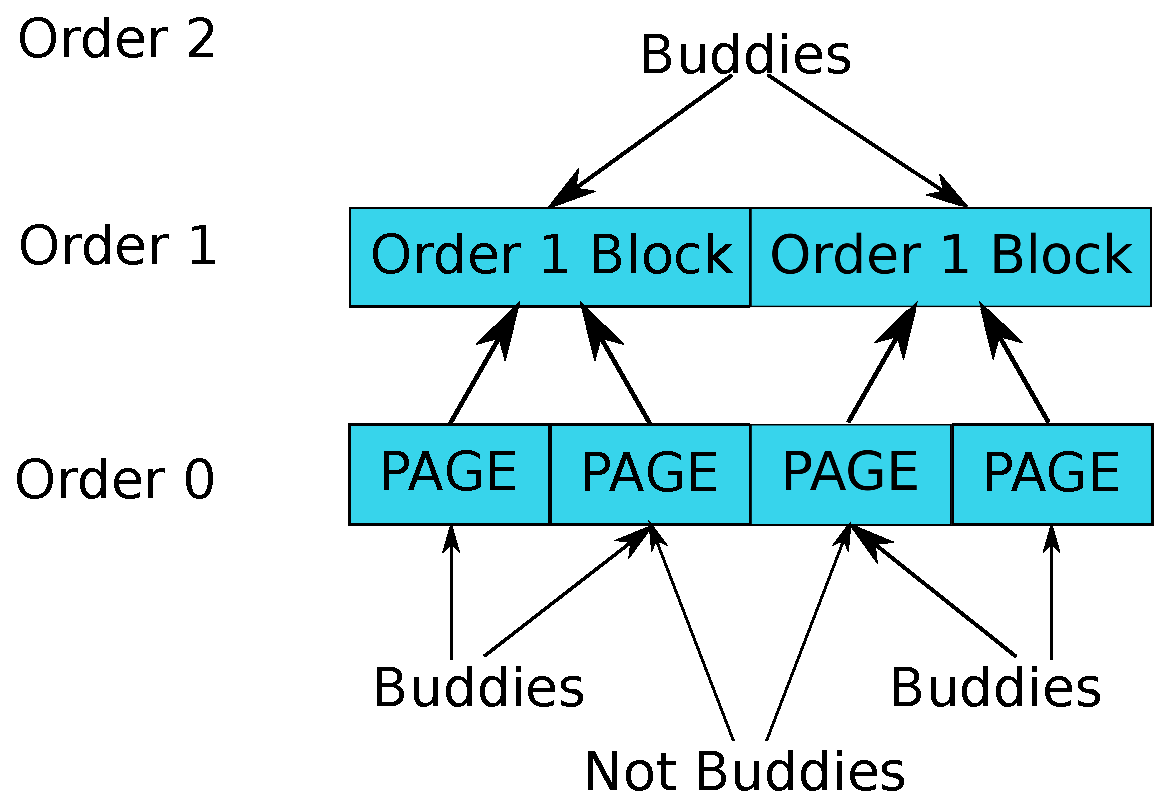
\includegraphics[width=.9\linewidth]{buddy-buddies}

\end{frame}
